\subsubsection{Mobiiliverkko}
\begin{figure}[htb]
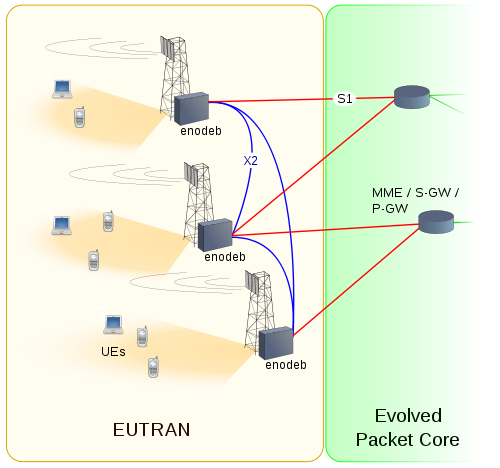
\includegraphics[scale=0.5]{EUTRAN}
\caption{Mobiiliverkon rakenne} \label{mobiarch}
\end{figure}

Tässä tutkielmassa käsiteltävät reuna-arkkitehtuurit sisältävät yhdistävänä tekijänä tavoitteen toimia mobiiliverkon yhteydessä. 
Täten reuna-arkkitehtuurien suunnittelupäätöksiä tarkasteltaessa on tarpeen ymmärtää mobiiliverkon osat yleisellä tasolla.
Yksinkertaisuuden vuoksi tämän tutkielman puitteissa mobiiliverkoksi oletetaan LTE:n mukainen arkkitehtuuri, joka koostuu E-UTRAN tyyppisestä radioverkosta ja EPC tyyppisestä runkoverkosta.
Seuraavaksi käydään läpi mobiiliverkon arkkitehtuurin tämän tutkielman kannalta merkitykselliset osat ja toiminnot.

Korkealla tasolla mobiiliverkko koostuu kahdesta osasta: radioverkosta ja runkoverkosta. 3GPP kehittämässä LTE standardissa radioverkon sisältävä osuus on nimeltään E-UTRAN (Evolved UMTS Terrestrial Radio Access Network) ja runkoverkon osuus on nimeltään EPC (Evolved Packet Core). Kuva \ref{mobiarch} sisältää yleisnäkymän mobiiliverkon osiin sekä niiden välisiin yhteyksiin.

E-UTRAN tehtävänä on toimia rajapintana asiakaslaitteen ja EPC:n välillä. Asiakaslaitteiden suuntaan E-UTRAN tarjoaa radioyhteyden ja yhtenä E-UTRAN tehtävänä onkin radioresurssien hallinointi. 
E-UTRAN sisältää verkon puolella pääasiallisena toimijana eNodeB tyyppisiä tukiasemia \cite{etsieutran}, myös muutamia erilaisia tukiasema variaatioita olemassa, mutta ne jätetään käsittelemättä.
Tukiasema on asiakaslaitetta lähimpänä sijaitseva funktionaalinen verkon osa ja sen seurauksena se on houkutteleva kohde reunalaskenta ratkaisuille. Tukiasemaa voikin ajatella \textit{reunan} viimeisenä etappina ennen asiakaslaitetta. 

ENodeB:n tehtävänä on kommunikoida radioyhteyttä käyttäen asiakaslaitteen kanssa ja välittää molemminsuuntaista liikennettä EPC:n (Evolved packet core) suuntaan. ENodeB on EPC:n suuntaan yhteydessä S1 rajapinnan kautta. ENodeB:t ovat myös yhteydessä toisiinsa X2 rajapintaa käyttäen. 
X2 rajapintaa käytetään tukiasemien väliseen kommunikointiin, jonka tarkoituksena on mahdollistaa muun muassa handoverin yhteydessä tehtävää asiakaskontekstin siirtoa ja erinäisiä muita hallinnollisia toimintoja \cite{3gpplte}.  
Handoverilla tarkoitetaan asiakaslaitteen radioyhteyden siirtoa toiselle tukiasemalle. Handover käsitellään tarkemmin kappaleessa \ref{livemigraatio}.

Mobiiliverkossa käytävä kommunikaatio voidaan jakaa kahteen kerrokseen: kontrollikerrokseen ja tietoliikennekerrokseen.
Kontrollikerroksella välitettävät viestit ovat tarkoitettu hallinnollisiin toimitoihin mobiiliverkon sisällä. 
Tietoliikennekerros välittää asiakkaan tietoliikennettä internetin ja asiakaslaitteen välillä.

EPC koostuu kolmesta alikomponentista, jotka ovat MME (Mobility Management Entity), SGW (Serving Gateway) ja PDN GW (PGW, Packet data network gateway) \cite{etsilte}.
SGW eli palveluyhdyskäytävä on asiakaslaitteen kiintopiste EPC:n sisällä.
SGW reitittää asiakkaan tietoliikenteen PGW:n ja E-UTRAN välillä. 
PGW:n tehtävänä on toimia IP tason reitittimenä EPC:n ja ulkoisen verkon välillä. 
PGW toimii asiakkaan ulkoverkon IP yhteyksien väylänä, kuin verkkokorttina. 
MME on EPC:n hallinnollinen komponentti ja se toimii ainoastaan kontrollikerroksessa. Sen tehtäviin kuuluu muun muassa asiakaslaitteiden identifiointi ja handovereihin liittyvät tilapäivitykset.
\cite{3gppepc}